\documentclass[12pt,oneside,abbrevs,dtc,mscres,neuro,notimes,logo]{styles/infthesis}

\usepackage{reportpackages}
\usepackage[strict]{changepage}
\usepackage{longtable}
\usepackage{rotating}
\usepackage[morefloats=7]{morefloats}

\mathtoolsset{showonlyrefs=false}

\renewcommand\theFancyVerbLine{\normalsize\arabic{FancyVerbLine}}

% Project Details

\title{Graph Theory as an Alzheimer's Disease Diagnostic Instrument in the Context of Functional Brain Connectivity}
%\title{Analysis of Functional Brain Connectivity using Graph Theory in Alzheimer’s Disease}
%Graph Theory as an Alzheimer's Disease Diagnostic Instrument in the Context of Functional Brain Connectivity 
%Applied to Functional Brain Connectivity as a Disease Prediction 
\author{Dragos Stanciu}
\submityear{2014}
\date{\today}


%\newacro{ACRNM}{Description}
\newacro{AD}{Alzheimer's Disease}
\newacro{ANOVA}{analysis of variance}
\newacro{BCT}{Brain Connectivity Toolbox}
\newacro{C}{average clustering coefficient}
\newacro{cBSS}{constrained blind source separation}
\newacro{CS}{control subjects}
\newacro{CSD}{cross-spectral density}
\newacro{DMN}{default mode network}
\newacro{DTI}{diffusion tensor imaging}
\newacro{dWPLI}{debiased weighted phase lag index}
\newacro{EEG}{electroencephalography}
\newacro{FC}{Functional Connectivity}
\newacro{FDA}{Functional Data Analysis}
\newacro{FIR}{Finite Impulse Response}
\newacro{fMRI}{functional magnetic resonance imaging}
\newacro{GE}{global efficiency}
\newacro{GLM}{Generalised Linear Model}
\newacro{IIR}{Infinite Impulse Response}
\newacro{ImC}{imaginary component of the coherence}
\newacro{L}{characteristic path length}
\newacro{LOOCV}{leave-one-out cross-validation}
\newacro{MCI}{Mild Cognitive Impairment}
\newacro{MEG}{Magnetoencephalography}
\newacro{MMSE}{mini-mental state examination}
\newacro{PLI}{phase lag index}
\newacro{PLV}{phase locking value}
\newacro{PS}{phase synchronisation}
\newacro{Q}{modularity}
\newacro{SD}{standard deviation}
\newacro{SMOTE}{Synthetic Minority Over-sampling Technique}
\newacro{SQUID}{superconducting quantum interference device}
\newacro{SVM}{support vector machine}
\newacro{SW}{small-world}
\newacro{t-SNE}{t-Distributed Stochastic Neighbour Embedding}
\abstract{
	One of the most common causes of dementia is \ac{AD}. \ac{MEG} is a neuroimaging technique that can monitor how neural oscillations are altered in patients suffering from this disorder. Graph theory is a framework that only recently has been applied to the study of structural and \ac{FC} in the human brain. This project aims to construct and compare functional connectivity graphs of healthy subjects and of patients suffering from \ac{AD} and \ac{MCI}. The debiased weighted phase lag index is used to quantify \ac{PS} between \ac{MEG} sensors. These partial results are used to build \ac{FC} graphs for each subject. A number of graph features such as clustering coefficients, modularity and \ac{SW} topology are compared between the three groups. Classifiers based on logistic regression and random forests are then trained using the computed graph metrics. Recordings of new subjects are assigned into one of the \ac{AD}, \ac{MCI} or \ac{CS} categories. A data processing pipeline that achieves the above was designed in the course of this project. A decrease of the \ac{SW} measure in \ac{AD} networks compared to \ac{CS} indicates a decline in network organisation. Poor sensitivity and specificity render the classifiers unsuitable in clinical settings.
}

% aims and objective
% background 
% methodology - main methods
% results - main findings
% conclusions - main conclusions 



% Extra Package Commands
\begin{document}
  \begin{preliminary}
    % Title Page
    \shieldtype{1}
    \maketitle
    \pagenumbering{roman}
    % Preamble
    \begin{acknowledgements}

I would like to express my gratitude to my supervisor, Dr Javier Escudero Rodriguez, for his constant support offered during the course of this project. I would also like to thank the collaborators from the Centre for Biomedical Technology at the Technical University of Madrid for providing the data and for their advice on addressing various issues when working with \ac{MEG} recordings.  

\end{acknowledgements}

    \standarddeclaration
    \input{sections/misc/dedication}
    \tableofcontents
    \listoffigures
    \listoftables
    %\listofacronyms
  \end{preliminary}

  \acresetall
  \pagenumbering{arabic}
  % Chapters
  \chapter{Introduction}

% 500-750 words

% context in which research took place
% why is the subject important
% key participants




\section{Motivation}
% why was this research carried out; application of machine learning to clinical setting...
\ac{AD} is the most frequent cause of dementia \autocite{Cummings2004}. Global costs are expected to have a remarkable growth as predictions show that by the year 2050, 1 out of 85 people will suffer from the disease \autocite{Brookmeyer2007}. \ac{MCI} is a key pre-stage of \ac{AD} \autocite{Morris2001}. Early diagnosis of this stage using inexpensive biomarkers would allow a larger number of patients to start treatments in advance. This may significantly delay disease onset \autocite{Cummings2004}.

Network analysis of neurodegenerative disorders is a young research field which has already shown promising results in disease diagnosis and progression \autocite{Zhou2010, Rowe2010DCM}. \ac{MEG} is a neuroimaging technique that can help find differences between neural patterns in the diseased brain and healthy brain \autocite{Stam2010}. Graph theory is a well-established framework that has the potential to standardise interpretation of neuroimaging results \autocite{Stam2010}. 

Existing results are inconsistent with respect to certain methodologies \autocite{Tijms2013}. This piece of research aims to supplement the current \ac{AD} research literature by employing promising techniques from three areas of interest: signal processing, graph theory and machine learning. 

\section{Objectives}
\label{sec:objectives}

The present data analysis project aimed to answer the following research question: 

\begin{center}
	{\textbf{What are the identifiable differences in functional brain connectivity between populations of \ac{AD}, \ac{MCI} and \ac{CS}?}}
\end{center}
The partial objectives of the project were defined in the original proposal \autocite{Stanciu} as follows:


\begin{description}
\item[Signal Processing] \hfill \\
  Compute correlations between pairs of \ac{MEG} sensors
  \item[Graph Analysis] \hfill \\
  Compute functional connectivity graphs and graph measures
  \item[Classification] \hfill \\
  Train classifiers using graph measures as features to assign recordings of new subjects in one of the \ac{AD}, \ac{MCI} or \ac{CS} categories
\end{description}
% end Objectives

\section{Achievements}

A modular data processing pipeline has been created which is able to take \ac{MEG} recordings as input and make predictions about which of the \ac{AD}, \ac{MCI} or \ac{CS} groups the signals originated from.

Brain connectivity graphs were created and graph measures were extracted from them. Classifiers were trained on these measures with the purpose of disease prediction.

Statistical analysis showed that for certain pipeline settings, results were not significant. Nevertheless, an easy to customise framework is in place and future methodological refinements should produce better results.

% end Achievements

\section{Outline}

% what topics are going to be discussed in each chapter and how each chapter related to each other; ROADMAP 

\begin{itemize}
	\item \textbf{Chapter 2} contains background research for better understanding of the scope of the project. Brief presentations of \ac{AD} and \ac{MEG} are provided in the beginning sections. These are followed by a description of graph theory concepts and a review of recent studies applying graph theory in the context of functional brain connectivity.

	\item \textbf{Chapter 3} describes the signal processing, graph theory and classification stages of the pipeline used to address the research question in Section~\ref{sec:objectives}. Techniques used for each of the three modules are explained. 

	\item \textbf{Chapter 4} presents the results of this project. These are comprised of extracted graph measures, statistical analysis performed on these values and performances of classification methods.

	\item \textbf{Chapter 5} evaluates the findings and discusses project limitations. 

	\item \textbf{Chapter 6} compares deliverables with initial project objectives and suggests avenues for future research.   
\end{itemize}
% end Outline

\section*{Conclusion}

This chapter described why research in \ac{AD} is important and outlined the project objectives. The next chapter describes key concepts needed for a better appreciation of the research methods used in this project. 









  \chapter{Background}
% 2000 words
	The project involved analysis of brain connectivity graphs computed from \ac{MEG} recordings. The following chapter depicts background knowledge needed for a better understanding of chosen methodologies.

	% AD - complete
	\section{Alzheimer's Disease}
	Increasing evidence points that the accumulation of beta-amyloid (A\(\beta\)) plaques in brain tissue is the most likely cause of \ac{AD} \autocite{Cummings2004}. Neuronal death is believed to be an effect of this increase in plaques. The only precise way of diagnosing \ac{AD} is by post-mortem examination of cortical tissue, but this is useful only in disease confirmation after death \autocite{Khachaturian1985}. Treatment in earlier phases of the disease can prove beneficial in delaying disorder symptoms. There are four main stages of \ac{AD}: \ac{MCI}, Mild and Moderate \ac{AD} and Severe \ac{AD}. In the \ac{MCI} stage, the patient experiences memory loss as a main symptom \autocite{Morris2001}. An area of disease diagnostic that shows promising results is represented by neuroimaging biomarkers \autocite{Weiner2013,Filippi2011,Sperling2011}. 


	% MEG 
	\section{The Physics of \ac{MEG}}
		\ac{MEG} is a noninvasive neuroimaging technique that measures perturbations occurring in the magnetic field produced by populations of neurons in the brain \autocite{LopesdaSilva2013}. Figure~\ref{fig:MEGsignal} shows that magnetic fields are generated by neuronal currents and picked up by the \ac{MEG} sensors. The main advantage of this technology is the high temporal resolution (1-100 Hz). Compared to \ac{EEG} that records electrical impulses at the scalp level, \ac{MEG} is more precise as magnetic signals suffer less distortion by the scalp and skull \autocite{LopesdaSilva2013}. 

		% ?? REFERENCE IF PERMISSION GRANTED
		\begin{figure}
		    \centering
		    \includegraphics[width=0.8\textwidth]{magneticfield-origin}
		    \caption{Magnetic fields are generated by the electrical activity of neurons (adapted from \textcite{Washington}).}
		    \label{fig:MEGsignal}
		\end{figure}

		% brief history of MEG
		% Explain Physics of MEG (vid); 2 physical phenomena are at the core of MEG technology; one is superconductivity and the other is quantum interference. explain them.
		The main technological achievement that lies at the foundation of \ac{MEG} technology is the \ac{SQUID} \autocite{Vrba2001}. This is a very sensitive magnetic detector based on two physical phenomena: superconductivity and quantum tunnelling. It was first used by \textcite{Cohen1972} in the context of a single-channel recording. Today's \ac{MEG} systems can have several hundreds of channels, where each channel corresponds to its own \ac{SQUID} \autocite{Vrba2001}.

		% MEG noise sources
		There are also several disadvantages of \ac{MEG} that one should be aware of. In contrast to having high temporal resolution, \ac{MEG} also has low spatial resolution (order of millimetres or centimetres) \autocite{LopesdaSilva2013}. One of the most pervasive problems in \ac{MEG} recordings is additive noise. Sources of noise can come from the exterior of the sensor helmet such as cardiac artefacts \autocite{Jousmaki1996} and power lines \autocite{Keshtkaran2014} or from the interior such as ocular artefacts caused by blinks \autocite{Jousmaki1996}. These should be minimised in the preprocessing stage of any analysis. The final problem mentioned here is the volume conduction problem that appears when activity from the same source is registered by multiple \ac{MEG} sensors because of their proximity \autocite{LopesdaSilva2013}.

		
	\section{Resting-State Synchronisation}
	% theory - Default Mode Network paper (no graphs)
	Traditionally, \ac{MEG} signals can be grouped in a number of frequency bands: infraslow (<0.2 Hz), \(\delta\) (0.2-3.5 Hz), \(\theta\) (4-7.5 Hz), \(\alpha\) and \(\mu\) (8-13 Hz), \(\beta\) (14-30 Hz), \(\gamma\) (30-90 Hz) and high-frequency oscillations (>90 Hz) \autocite{LopesdaSilva2013}. When populations of neurons share the same firing patterns, neural oscillations arise. Cognitive functions such as memory are believed to rely on these synchronisation patterns between different regions of the brain \autocite{Schnitzler2005, Gusnard2001}. The \ac{DMN} is a network of brain regions that is believed to be active during resting states, when the person is not actively engaged with a certain task \autocite{Raichle2001}. Since the introduction of this hypothesis, resting-state studies have been successful in identifying correlations in the same brain regions across subjects \autocite{Damoiseaux2006,Beckmann2005,Andrews-Hanna2010}.

	As \ac{AD} affects memory, the next step was to try to find differences between the healthy population and patients. Several studies have found significant differences between these groups, where connectivity in \ac{AD} patients was lower than in control subjects \autocite{Stam2006,Greicius2004,Sheline2010}. The next section introduces graph theory as a relatively new paradigm for brain network analysis \autocite{Stam2012}.

	\section{Connectivity Graphs}
	% network analysis is a new way to compare the disruptions
	Quantitative analysis of brain networks can be obtained using graph theory \autocite{sporns2011networks}. Mapping states of biological networks to corresponding graph measures would be instrumental in disease diagnosis and development.

	A graph is a structure composed of a set of nodes or vertices and a set of edges. The nodes are connected by the edges. When referring to brain graphs, nodes are mapped to anatomical regions and edges specify a connectivity function. This function can be either structural or functional. The structural function describes the anatomical connections of the nervous system and employs \ac{DTI} and tractography \autocite{Jones2011}. \ac{FC} depicts neurophysiological patterns and is explored using \ac{MEG}, \ac{EEG} or \ac{MEG} technologies. Figure~\ref{fig:structfunctnetworks} shows a high-level scheme of extracting graphs from brain signals. Particular attention should be given to \textit{Step 2}, where the association between nodes is computed. In \ac{FC}, the synchronisation measure just describes statistical correlations between different brain regions and makes no statement about underlying causal effects \autocite{sporns2011networks}. 

	\begin{figure}
		    \centering
		    \includegraphics[width=0.95\textwidth]{structfunctnetworks}
		    \caption{Structural and functional brain networks (from \textcite{Bullmore2009}). Step 1 implies identification of graph nodes. This consists of anatomical regions in case of \ac{DTI} and electrodes in case of \ac{EEG} or \ac{MEG}. Step 2 computes a correlation measure between nodes. Step 3 creates an association matrix which holds the correlation strengths between pairs of vertices. Graph measures are computed in the final step.}
		    \label{fig:structfunctnetworks}
	\end{figure}   

	\section{Graph Theory}
	This sections aims to introduce a number of graph features relevant to the current study. A comprehensive review of more complex measures can be found in \autocite{Rubinov2010}.

	Node degree is one of the simplest graph measures. This is given by the number of edges that link a node to the rest of the graph. Another basic graph measure is node centrality. This refers to the number of shortest paths between the other pair of nodes in the network that pass through a specific node. High-centrality measures are critical for fast communication. Network hubs are vertices with either high centrality or high degree. Figure~\ref{fig:graphmeasures} provides an overview of some of the measures.  
	
	The clustering coefficient quantifies local segregation. It refers to how densely connected is a node relative to its neighbours. A high value for this measure indicates that a cluster has been found. The average shortest path length, also called the \ac{L}, is calculated by taking the average number of edges in the shortest paths between every node pair in the graph. This measure can also be found under the name of unnormalised path length. The normalised path length is obtained by dividing \ac{L} by the average path length of a random graph. Random graphs are introduced in the next subsection. 

	A graph is said to have high modularity if it is formed of subgraphs (modules) that display high intraconnectivity and low interconnectivity (connection between subgraphs). 

	\begin{figure}
		    \centering
		    \includegraphics[width=0.8\textwidth]{graphmeasures}
		    \caption{Graph measures (adapted from \textcite{Stam2012}). The red node in the \textit{degree} graph has a degree of three. For the \textit{shortest path graph}, a minimum of four edges need to be traversed from the red node to the blue node which yields a shortest path of four. Four modules can be seen in the \textit{modularity} graph.}
		    \label{fig:graphmeasures}
	\end{figure}   

	\textcite{Watts1998} introduced the idea of "small-world" networks which maintain an equilibrium of high clustering and short paths. Brain networks have been hypothesised to posses this property as a consequence of needing to balance infrastructure costs (building neural paths and maintaining them) and high connectivity between brain regions. Fast local computation and integration of information is achieved using the \ac{SW} topology \autocite{Bullmore2009}. Figure~\ref{fig:smallworld} compares the \ac{SW} network with two other networks.

	\begin{figure}
		    \centering
		    \includegraphics[width=0.8\textwidth]{smallworld}
		    \caption{Basic network types (from \textcite{Watts1998}). Each node of a network is initially connected to its four neighbours. The network is highly clustered and the majority of path lengths between nodes are high. With a probability \textit{p}, edges are disconnected and reattached to a random node. For \textit{p}=1, all of the edges will be reconnected which would result in a random network. This network type lost the high clustering property. For value of \textit{p} between 0 and 1, the network maintains the high clustering quality and depicts small path lengths.}
		    \label{fig:smallworld}
	\end{figure}   

	
	\section{Network Measures as Biomarkers in AD}
	% AD studies (from section 1.2: Graph analysis of AD brain...)
	Analysis of \ac{AD} brain networks using graph theory is a relatively recent research endeavour. Two reviews that describe studies that focused exclusively on \ac{AD} are the ones by \textcite{He2009} and \textcite{Xie2011}. Findings of 13 studies that explored graph metrics in \ac{AD} were listed in the review by \textcite{Tijms2013}. They found that connectivity decreases in \ac{AD} graphs. Common graph characteristics were identified by most of the studies, but there are cases where properties are inconsistent across results.

	Previous studies reported a decline in clustering coefficients in \ac{AD} graphs \autocite{He2009,DeHaan2012a}. The research by \textcite{Stam2004} was one of the first to show that brain networks in healthy subjects have the \ac{SW} property. All studies reviewed in \textcite{Tijms2013} reported that \ac{AD} networks possess the \ac{SW} property and 3 out of 13 studies described a decline in the \ac{SW} value in \ac{AD} networks, with a possible explanation of path length increase. The reported normalised path lengths in \textcite{Tijms2013} were inconsistent. The connection between path length and \ac{SW} property in \ac{MCI} and \ac{AD} patients was superficially investigated in the past \autocite{Tijms2013}. 
	Modularity in \ac{AD} was explored in only a single study which found a fewer number of modules in \ac{AD} networks \autocite{DeHaan2012b}. In the same study, modularity in the \(\theta\) band was increased.    

	Result incompatibilities between studies may be caused by lack of standardised techniques for creating \ac{FC} graphs \autocite{Tijms2013}. Another possible limitation is the small sample sizes employed in the studies. For research that aims to compare three groups such as the one in this project (i.e.\ \ac{AD}, \ac{MCI} and \ac{CS}), larger sample sizes are needed.  

	% we look at global measures -> global approach to characterise networks

	\begin{figure}
		    \centering
		    \includegraphics[width=0.9\textwidth]{MLbraingraphs}
		    \caption{Scheme for predictive analysis using brain graphs (from \textcite{Richiardi2013}). In a), imaging data is arranged in regions of interest with each region having corresponding time series. b) A graph is computed from the signals in which vertices correspond to brain regions and edges represent correlations between these regions. c) The graphs are organised in vector structures. d) The vectors are used as input for machine learning algorithms. e) Visualisation of interesting patterns is performed so results can be better interpreted. f) Model evaluation is done in the last stage to assess algorithm quality.}
		    \label{fig:MLbraingraphs}
	\end{figure}

	In addition to studies that looked only at comparing network measures in \ac{AD}, another category distinguishes itself by trying to use machine learning techniques on computed graph features and subsequently performing classification of individuals \autocite{Jie2014,Chen2011,Zhou2011}. The goal is to bring this research into clinical settings for illness diagnosis purposes. A pipeline schema of a project employing graph analysis in a machine learning setting can be seen in Fig.~\ref{fig:MLbraingraphs}. 

	% bit of background about past papers using ML for classification
	% utility of graphical metrics as diagnostic markers

	This project brought together graph analysis of \ac{FC} networks and classification techniques with the aim of furthering research into network-based diagnosis procedures in \ac{AD}.
	% then: in this project we applied graph analyis to compare \ac{FC} networks between AD, MCI and controls. we examined 

\section*{Conclusion}
	This chapter started by describing \ac{AD} and why research in this area is important. Afterwards, an overview of \ac{MEG} was provided as this is the imaging technique used to acquire the data for this project. Lastly, an overview of the state-of-the-art research in graph analysis applied to \ac{AD} was presented. The next chapter describes the specific techniques used to tackle the problem of finding dissimilarities between \ac{AD} patients and healthy people.
  % 1000 - 2000 words
% justify process by which the research question was answered
% justify each decision! state what each option is, why you made the choice that you did, why you rejected those not used
% justify why the chosen methods were selected as the most appropriate
% reference advantages/disadv of methods with relevance to my choice

\chapter{Methodology}

	\section{Pipeline Overview}
	
	Figure~\ref{fig:pipeline} summarises the data processing pipeline developed for finding differences in \ac{FC} between the \ac{AD}, \ac{MCI} and \ac{CS} groups. Justifications for chosen methods in different stages are found in corresponding sections.
	
	% pipeline figure here
	\begin{figure}
	    \centering
	    \includegraphics[width=1\textwidth]{pipeline}
	    \caption{Processing pipeline illustrating different stages of data manipulation.}
	    \label{fig:pipeline}
	\end{figure}
	%\includegraphics[scale=0.7]{pipeline.eps}

	In the signal processing stage, \ac{MEG} signals are first filtered into specific bands of interest. The frequency spectrum is then computed for these filtered signals which is then used to perform connectivity analysis between the channels. The connectivity values are saved into matrices which are then used as adjacency matrices in the graph analysis stage. Graph measures are computed from the created networks which are then combined to form feature vectors. Statistical analysis is done to verify differences between each of the \ac{CS}, \ac{MCI} and \ac{AD} groups. The graph feature vectors are finally used as training data for a number of classifiers with the goal of assigning unseen data into one of the studied groups.

	% end Overview

	\section{Dataset}
	The project made use of the same dataset employed in \textcite{Escudero2011a}. \ac{MEG} signals were recorded from a total of 80 subjects in resting-state, with their eyes closed. The data was acquired at the Centre for Biomedical Technology of the Technical University of Madrid using a 148-channel whole-head magnetometer (MAGNES 2500 WH, 4D Neuroimaging). Figure~\ref{fig:4d148} shows the layout of the 148 channels. The recordings are five minutes long, collected at a sampling frequency of 169.54 Hz. The \ac{MMSE} is a test that reflects the cognitive abilities of a subject \autocite{Folstein1975}. Such test scores have also been gathered from all participants. The number of subjects in each group, mean age with \acp{SD} and \ac{MMSE} scores can be viewed in Table~\ref{tab:dataset}.
	
	\begin{table}
		\centering
	    \begin{tabular}{llll}
	    \hline
	    Group                 & No of subjects & Mean age (\(\pm\) SD)   		 & MMSE         \\ \hline
	    CS 					  & 26             & 71.77 \(\pm\) 6.38 years                    & 28.88 \(\pm\) 1.18 \\
	    MCI                   & 18             & 74.89 \(\pm\) 5.57 years                    & 25.67 \(\pm\) 1.81 \\
	    AD                    & 36             & 74.06 \(\pm\) 6.95 years                    & 18.06 \(\pm\) 3.36   \\
	    \end{tabular}
	    \caption{Statistics of subjects used in this study}
	    \label{tab:dataset}
	\end{table}

	\begin{figure}
	    \centering
	    \includegraphics[width=0.7\textwidth]{4d148.png}
	    \caption{Layout of the 148 channels across the subject's head. Image from the FieldTrip toolbox \autocite{Oostenveld2011}.}
	    \label{fig:4d148}
	\end{figure}

	The provided dataset contained two sets of recordings. The first set consisted of the raw \ac{MEG} recordings which were subjected to routine preprocessing methods (see \textcite{Escudero2011a} for details), while the second set was a subset of the former and was made up of a number of 10s epoch files. These epochs were selected such that obvious ocular artefacts were not present with the help of an amplitude thresholding technique \autocite{Hornero2008}. In addition to this, the cardiac artefact was removed from these recordings with a constrained blind source separation method described in \textcite{Escudero2011b}.

	The current analysis was done on the second set of recordings cleaned of ocular and cardiac artefacts. 

	% end Dataset
	
	\section{Signal Processing} 
	
	This section describes the first part of the processing pipeline which takes as input the 10s epochs and returns connectivity matrices. Figure~\ref{fig:SPpipeline} condenses the tasks involved. The FieldTrip Matlab signal processing toolbox was used for implementation \autocite{Oostenveld2011}. A significant amount of time was spent developing this component as previous experience with signal processing was absent prior to the start of the project. 
	
		\begin{figure}
		    \centering
		    \includegraphics[width=0.7\textwidth]{phasesync}
		    \caption{Signal processing pipeline (from \textcite{Varela2001}). Raw \ac{MEG} recordings are filtered into the bands of interest. Frequency analysis is used to compute the phase of the signals. Connectivity measures employ this information to establish the level of synchronisation.}
		    \label{fig:SPpipeline}
		\end{figure}

		\subsection{Data Preprocessing}
		
		Scripts were written to check the integrity of the recordings so that invalid values or other inconsistencies across the files would not affect the next stages of the pipeline. No obvious problems were found with the given data.

				
			\subsubsection{Baseline Correction}
			It is important to note that the continuous (DC) offset is present in \ac{MEG} recordings. As it is desirable for the signals to have a variation around zero, subtraction of the mean registered value across each channel is a common preprocessing step \autocite{Gross2013}. As this is an offline analysis, the subtracted mean is computed across the whole epoch so as not to bias the mean, i.e.\ computing the mean using only the first few samples.

			\subsubsection{Filtering}
			Filtering is the process by which a signal of interest is extracted by attenuating unwanted components from the original signal \autocite{smith1997scientist}. The study aimed to inspect \ac{FC} in the following physiologically relevant bands:
			
			\begin{itemize}
				\itemsep0em
  				\item \(\delta\): 0.5 - 4 Hz  
  				\item \(\theta\): 4 - 8 Hz 	 
  				\item \(\alpha\): 8 - 13 Hz 
  				\item \(\beta\): 13 - 30 Hz 
				\item \(\gamma\): 30 - 45 Hz
			\end{itemize}

				%% ?? take it out of the text filtered epoch??
			In order to restrict connectivity analysis to a specific band, filtering was performed similarly to the study by \textcite{Stam2009}. This was done using FieldTrip's \textit{ft_preprocessing} function. Epochs were band-pass filtered for each of the above bands using a \ac{FIR} filter which effectively reduced the strength of signals outside the specified frequency intervals. An \ac{FIR} filter was chosen over an \ac{IIR} filter as the former exhibits a linear phase response whereas the latter distorts the phase of the signal \autocite{Gross2013}. Preserving the phase is crucial for correctly computing \ac{PS}. Although the filter should not in theory affect the phase, the attenuation was applied in both forward and reverse directions as an extra precaution. The filter used a Hamming window, a common and popular windowing function and a filter order of 560 to ensure that the transition from the pass to the stop band is abrupt.   

			A problem that one should be aware of is the power line interference that affects neural recordings at 50 Hz and harmonic frequencies \autocite{Keshtkaran2014}. As the highest frequency oscillations studied here are in the interval 30-45 Hz, this does not constitute a problem since the interference is high-pass filtered.

			Another problem when performing filtering is the occurrence of edge effects. These arise at the beginning and end of the epoch during the filter pass. The standard method to reduce this problem is padding the signal with extra data. A series of tests were carried out to see if padding the \ac{MEG} signals would cause a significant difference in the phases of the signals. 

			In order to better understand how the phase of a signal is obtained, the Hilbert transform is introduced in the next subsection.

		\subsection{Frequency Analysis}

			\subsubsection{Hilbert Transform}
			At the foundation of \ac{PS} measures lies the instantaneous phase. After filtering the data in a particular frequency band, the instantaneous phase at any given point in time can be extracted using the Hilbert transform \autocite{LeVanQuyen2001}. The initial time series signal \(x(t)\) can be written in analytic form as in Eq.~\ref{eq:analytic-signal}.

			\begin{equation}\label{eq:analytic-signal}
				z(t) = x(t) + i\tilde{x}(t)
			\end{equation}
			
			where \(\tilde{x}(t)\) is the Hilbert transform of \({x}(t)\):

			\begin{equation}\label{eq:hilbert-transform}
				\tilde{x}(t) = \frac{1}{\pi} p.v. \int_{-\infty}^{\infty} \frac{x({t}')}{t-{t}'}d{t'} 
			\end{equation}
			(\textit{p.v.}\ is the Cauchy principal value). The Hilbert phase is:
			
			\begin{equation}\label{eq:hilbert-phase}
				\Phi_{x}^{H}(t) = \arctan \frac{\tilde{x}(t)}{x(t)}
			\end{equation}

			Unpadded and padded signals were filtered into the bands of interest and the Hilbert transform was computed to obtain the instantaneous phase. The chosen padding was symmetric padding which follows the trend of the signal. In figure~\ref{fig:hilbert-difference} the phase difference between the padded and unpadded signals for an \(\alpha\) band filtered epoch can be observed.    

			%\input{/home/dragos/DTC/MSc/SummerProject/report/images/HilbertPhase.tex}  
			% figure: Hilbert Phase Difference
			\begin{figure}
			    \centering
			    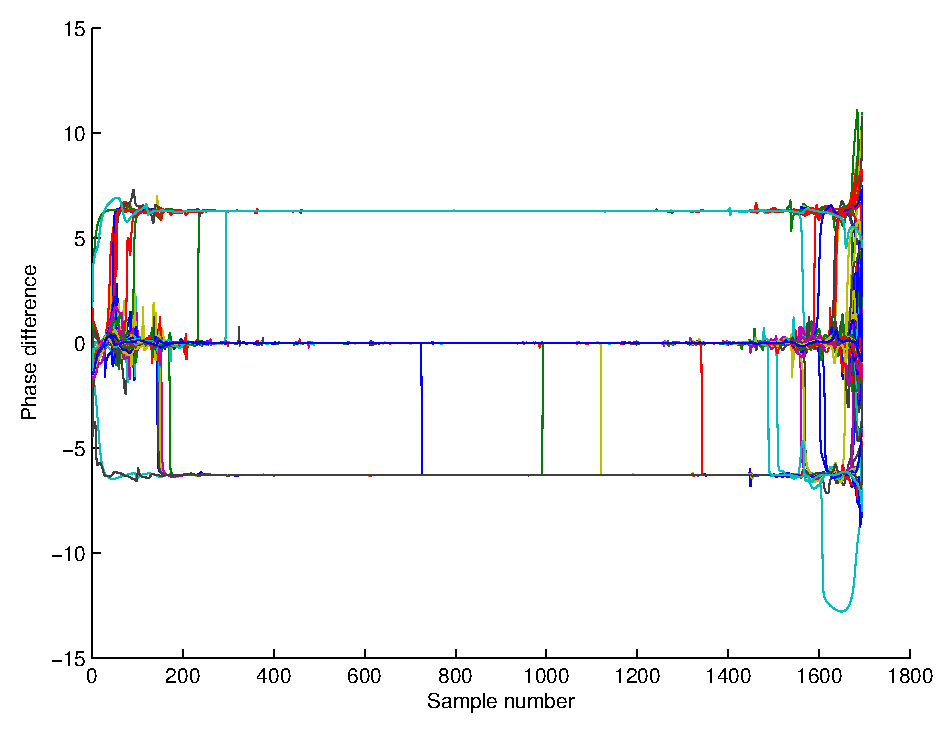
\includegraphics[width=0.8\textwidth]{HilbertPhaseDiff}
			    \caption{Subtracted phases of a padded and unpadded filtered epoch in \(\alpha\) band.}
			    \label{fig:hilbert-difference}
			\end{figure}	

			Small fluctuations of the phases occurred at the edges of the signal. This is expected because of edge effects. Visual inspection of similar phase differences in different epochs revealed similar fluctuations which were deemed insignificant to have an impact on the results. It was decided that signal padding shall not be applied.

			\subsubsection{Frequency Spectrum Estimation}
			% Welch's method and tapering	
			\ac{PS} measures require phase information which can be obtained from prior computation of the frequency spectrum. This is done by taking the Fourier transform of the given signals, which returns a series of complex numbers where the imaginary part comprises phase information. In order to reduce the amount of noise in the estimation of the frequency spectrum, Welch's periodogram method was employed \autocite{Welch1967}. The original 10s epochs were split into 2s segments with \(50\%\) overlap. These segments were then filtered into the bands of interest.

			Windowing functions, also called tapers, are multiplied with the data prior to spectral calculation to control frequency smoothing. For frequency bands below 30 Hz (\(\delta\) - \(\beta\)) it is sufficient to use only a single Hanning taper whereas for analysis in the \(\gamma\) band (30-45 Hz), multiple tapers should be used to improve frequency smoothing \autocite{Mitra1999,Percival1993}. In consequence, for the \(\gamma\) band, discrete prolate spheroidal sequences (Slepian sequences) were used as tapers with a smoothing box of \(\pm\)4 Hz \autocite{Slepian1978,Hoogenboom2006}. 

			For each 2s segment, spectral density was obtained via FieldTrip's \textit{ft_freqanalysis} function which facilitated tapering and Fourier analysis. The spectral estimates acquired in this stage were then used in connectivity analysis.

		\subsection{Connectivity Analysis}
		Connectivity measures try to quantify the degree of coupling between two signals. In the context of brain connectivity, these methods can be classified in two main categories: directed measures, which try to infer causal interactions between brain regions, and undirected measures which state the observed correlations \autocite{Friston1994}. As the goal of the project was to find differences in brain synchronisation of patients and controls during resting-state, where no particular causal interactions are sought, an undirected connectivity measure is a natural choice \autocite{Fallani2014}. The next step was to explore the available options and choose the ones most likely to yield positive results. In the past years, a series of methods were developed to address issues such as volume conduction and noise in recordings \autocite{Vindiola2014}. One of the most popular measure is the \ac{PLV} developed by \textcite{Lachaux1999} which is often used when comparing different measures \autocite{Aydore2013}. Another measure is the \ac{ImC} which is robust to spurious correlations caused by the volume conduction effect \autocite{Nolte2004}. A new measure that is gaining popularity is the \ac{dWPLI} created by \textcite{Vinck2011}. The study by \textcite{Vindiola2014} compared \ac{PLV}, \ac{ImC} and \ac{dWPLI} using simulations and found none of the measures to perform better than the others. In the present study, care was taken to develop a processing pipeline that would integrate with the FieldTrip toolbox so that different synchrony measures can be used effortlessly. This report presents the results obtained with the \ac{dWPLI} measure, but other techniques such as the \ac{PLV} and \ac{ImC} can be explored. 
		% also look at background for making this phrase cool? mention the stuff in the background at all?
			\subsubsection{Debiased Weighted Phase Lag Index}	
			The \ac{dWPLI} is an improved version of the \ac{PLI} developed by \textcite{Stam2007}. This newer technique aims to solve the problem of the \ac{PLI} not detecting changes in \ac{PS} in cases of weak coupling between the signals \autocite{Vinck2011}. It is also regarded as a method robust against volume conduction.

			\begin{equation}\label{eq:WPLI}
				{WPLI} \equiv \frac{|E\{\Im\{X\}\}|}{E\{\Im\{X\}\}} = \frac{|E\{|\Im\{X\}|sgn(\Im\{X\})\}|}{E\{|\Im\{X\}|\}}
			\end{equation}

			where \(\Im\{X\}\) is the imaginary component of the cross-spectrum between two signals \(x(t)\) and \(y(t)\). This measure returns values between 0 and 1, where 0 denotes no synchronisation and 1 indicates synchronisation. The debiased method was used in this study \autocite{Vinck2011}. Connectivity between each channel was computed using FieldTrips's \textit{ft_connectivityanalysis} function.


			% in figure the distribution of mean dWPLI values for each subject class are shown 

			%\begin{figure}
	    	%	\centering
	   		%	\includegraphics[width=0.8\textwidth]{dWPLIdistrib}
	   		%	\caption{Distribution of \ac{dWPLI} values. Mean values across subjects of each group are shown.}
	   		% \label{fig:dWPLIdistrib}
			%\end{figure}

			% distribution similar to Ortiz2012! so we can proceed to the next stage.   
			% ?? figure - histogram of dWPLI values 

		 The spectral density estimates computed in the frequency analysis step were used to calculate the connectivity values between all pairs of channels. As the recordings were made with a 148-channel \ac{MEG} machine, a \(148\times148\) matrix was computed illustrating the connectivity strength between each pair. A cell of this matrix corresponded to the correlation between the channel of the row and the channel of the column on which the cell was located. Employing Welch's method, intermediate connectivity values were computed for each 10s epoch. The final connectivity matrix of a subject was obtained by averaging the intermediate connectivity matrices across all epochs of a subject. Since the analysis was done for five bands of interest, five connectivity matrices were acquired for each subject. The matrices were then sent to the Graph Analysis module. 

	% end Signal Processing

	\section{Graph Analysis}

	This section describes the second part of the processing pipeline which takes as input the connectivity matrices from the signal processing unit and returns graph measures corresponding to the observed connectivity.

		\subsection{Constructing Brain Graphs}
		% absolute value because fieldtrip also returned negative connectivity values
		The \ac{dWPLI} connectivity matrices can be regarded as adjacency matrices of graphs modelling the subject's brain network activity for different frequency bands. Each \ac{MEG} channel can be seen as a node in the brain network, whereas entries in the matrix correspond to the strength between the nodes. For convenience, the connectivity matrix obtained in the previous stage can be written as \(W_{N \times N}\), where \textit{W} is a weighted symmetric matrix since \ac{dWPLI} is an undirected \ac{FC} metric. Although there is currently no optimal way of converting functional imaging data to graphs \autocite{StamReijneveld2007}, previous studies have consolidated certain procedures that one should take into account. 

		In the first instance, it was noticed that some negative values were obtained in the \ac{dWPLI} matrices. Consulting FieldTrip's documentation, this was normal as negative values denote anticorrelations between signals. The negative entries were replaced by their absolute values, as \textcite{Fallani2014} advise. The second step was to filter weak links as environmental noise or volume conduction may generate false correlations \autocite{Fallani2014}. A threshold \textit{X} must be chosen for deciding if an entry \(w_{ij}\) in \textit{W} is to be removed or kept. This threshold can either be an absolute threshold or a density threshold also called proportional threshold \autocite{Bullmore2011}. In the case of a simple absolute threshold, an arbitrary value is chosen which would remove edges when \(w_{ij}\) is smaller than that value. This is inappropriate as analysis would be restricted for that specific threshold \autocite{Bullmore2009}. Using a density threshold, only the top \textit{X\%} strongest links within the matrix are preserved. A varying density threshold has higher chances of finding topological differences between the networks in the three groups of interest. Care should be taken when choosing threshold values as filtering all links or keeping most of them would result in worthless analysis \autocite{Achard2007}. The five density thresholds chosen for \textit{X} are the following:

		\begin{equation}\label{eq:thresholds}
			X = \{0.05, 0.1, 0.15, 0.2, 0.3\}
		\end{equation}

		Thresholding each of the five frequency band connectivity matrices for five values produced 25 adjacency matrices per subject. A total of 2000 matrices were obtained as there are 80 subjects in the dataset.  
		Binarisation of the graphs is the step by which links that survived the thresholding process are set to unity and links that need to be removed are set to zero. The resulting matrices are treated as adjacency matrices for binary undirected graphs, where nodes \textit{i} and \textit{j} are connected if the \(w_{ij}\) entry is one. The motivation behind this step is that most graph measures used in the next stage operate only on binary graphs \autocite{Rubinov2010}.  

		\subsection{Graph Measures}

		Five graph features were calculated for each of the 25 brain graphs of a subject. The \ac{BCT} was used to compute these metrics \autocite{Rubinov2010}. Similar to the study by \textcite{Rudie2012}, the chosen measures for this step were global metrics. 

		\begin{description}
			  \item[average clustering coefficient (C)] \hfill \\
			  The local clustering coefficient of a node measures how densely connected is a node relative to the node's neighbours \autocite{Watts1998}.

			  \begin{equation}\label{eq:local-clust}
				C_i = \frac{2 e_i}{k_{i}(k_{i}-1)}
			  \end{equation}
			  where \(k_i\) is the number of neighbours of node \textit{i} and \(e_i\) is the number of edges between all of \textit{i}'s neighbours.

			  The \ac{C} is the sum of the local clustering coefficients divided by the total number of vertices. 
			  \begin{equation}\label{eq:avg-clust}
				\overline{C} = \frac{1}{n} \sum\limits_{i=1}^n C_i
			  \end{equation}
			  
			  \item[characteristic path length (L)] \hfill \\
			  \ac{L} is the average number of links in the shortest paths between every node pair in the graph.
			  \begin{equation}\label{eq:char-path-len}
				L = \frac{1}{n (n-1)} \sum\limits_{i\not=j} d(v_i, v_j)
			  \end{equation} 
			  where \(d(v_1, v_2)\) is the shortest distance between node \(v_1\) and  node \(v_2\).

			  \item[global efficiency (GE)] \hfill \\
			  \ac{GE} is the average inverse shortest path \autocite{Latora2001}. It is used instead of \ac{L} when networks have disconnected nodes \autocite{Fallani2014}.
			  \begin{equation}\label{eq:ge}
				GE = \frac{1}{n (n-1)} \sum\limits_{i\not=j} d(v_i, v_j)^{-1}
			  \end{equation} 
			  
			  \item[small-worldness (SW)] \hfill \\
			  The \ac{SW} index of a graph is defined as follows \autocite{Watts1998}:
			  \begin{equation}\label{eq:sw}		
				SW = \frac{ \frac{C}{ C_{rand} } }{ \frac{L}{ L_{rand} } }
			  \end{equation}
			  where \(C_{rand}\) and \(L_{rand}\) are the \ac{C} and \ac{L} of a random network.

			  Following the methodology described in \textcite{Rudie2012}, for each adjacency matrix, the computation of the \ac{SW} value was performed by generating a number of random networks that respected the number of nodes, node degree and edge distribution of the given adjacency matrix. In the referenced study, 100 random networks were generated for each subject network by disconnecting and randomly rewiring each edge of the given network using \ac{BCT}'s \textit{randmio_und_connected} function. The same method was applied in this study, with the observation that six random networks were generated for each matrix because of available computational resources. The average \ac{C} and \ac{L} of the created random networks became \(C_{rand}\) and \(L_{rand}\) in Eq.~\ref{eq:sw}. It is important to note that the \textit{randmio_und_connected} function, as the name suggests, maintains the connectedness property of the input graph. A connected graph is a graph where there is a path from any node to any other node.     

			  \item[modularity (Q)] \hfill \\
			  \ac{Q} quantifies to what extent can a network be divided into clearly separated clusters of nodes \autocite{Newman2003}.
			  \begin{equation}\label{eq:q}		
				Q = \sum\limits_{u \in M} \left[ e_{uu} - \left(\sum\limits_{v \in M} e_{uv} \right)^2 \right]
			  \end{equation}
			  where the graph is divided into nonoverlapping modules \textit{M} and \(e_{uv}\) is the proportion of edges connecting vertices in module \textit{u} with vertices in module \textit{v} \autocite{Rubinov2010}. 
			  For computing this measure, the \ac{BCT} \textit{modularity_und} function was used. For each graph, the function was executed 100 times as the \ac{Q} measure employs heuristics which can vary from run to run. The average of the 100 runs was taken as the final \ac{Q} for that graph.
		\end{description}

		After this stage, graph features have been computed for each subject, for all thresholds in Eq.~\ref{eq:thresholds}, for each frequency band of interest. 

	% end Graph Analysis

	\section{Statistical Testing}
	This section describes the statistical significance methods used to compare network measures between the groups.
		
		\subsection{Functional Data Analysis}
			The study by \textcite{Bassett2012} proposed \ac{FDA} to examine differences between schizophrenia patients and healthy controls. \ac{FDA} is a subfield of statistics used for curve comparison \autocite{Ramsay2005}. Each network measure computed in the previous section can be plotted as a curve, where the \textit{x} axis is the threshold value and the \textit{y} axis represent the value of the metric. 

			For between group comparisons, the nonparametric permutation test within \ac{FDA} can be used as follows: for each network measure, the average curves of \ac{AD}, \ac{MCI} and \ac{CS} groups are computed separately. Two groups, for example \ac{AD} and \ac{CS}, are chosen for comparison. The area \textit{A} between the curves of the chosen groups is calculated as in Eq.~\ref{eq:area}.

			\begin{equation}\label{eq:area}		
				A = \sum\limit_{i=1}^{5} |y_{AD}(X_i) - y_{CS}(X_i)|
			\end{equation}
			where \textit{i} goes through each threshold in Eq.~\ref{eq:thresholds}; \(y_{AD}\) and \(y_{CS}\) are the mean values of the network measure of all subjects in the \ac{AD} and \ac{CS} classes respectively. 

			Nonparametric permutation testing involves randomly reassigning without replacement the group identity of each subject within the classes chosen for comparison. In the \ac{AD} and \ac{CS} example, an \ac{AD} subject may be assigned to the \ac{CS} group and vice versa. The average curves of the two created pseudo-groups are then computed and the area \(A^\prime\) between these curves is calculated as in Eq.~\ref{eq:area}. The procedure is repeated for \(k=10000\) iterations to compile a set of \(k\) \(A^\prime\) values. The number of \(A^\prime\) values greater than \(A\) divided by the number of iterations \(k\) yielded the p-value of the true population difference, \(A\).  

			For each pair of groups (\ac{CS}-\ac{MCI}, \ac{CS}-\ac{AD}, \ac{MCI}-\ac{AD}), \ac{FDA} was performed for all measures, in all frequency bands.     

		% if I have time left.
		% http://www.mathworks.co.uk/help/stats/anova1.html
		% https://en.wikipedia.org/wiki/Shapiro%E2%80%93Wilk_test
		%\subsubsection{ANOVA}
		%	One-way \ac{ANOVA} was performed to cross-check the results from the \ac{FDA} analysis. One assumption the ANOVA test is that sample must be normally distributed. Shapiro-Wilk was used for that. 

	% end Statistical Testing

	\section{Classification}
	This section describes the last part of the processing pipeline which takes as input the graph measures from the graph analysis stage and uses multiple classification techniques to make predictions about which category a certain set of graph measures comes from.

	\subsection{Data Visualisation}
	\ac{t-SNE} is a dimensionality reduction algorithm that is able to take high-dimensional data as input and produce a 2D or 3D plot of the datapoints \autocite{Maaten2008}. It works by converting distances between data samples to probabilities and then attempts to minimise the Kullback-Leibler divergence between the joint probabilities of the initial high-dimensional data and the points in the new space with fewer dimensions. The technique is useful as it can show if samples of different classes can be separable in a linear or nonlinear manner. The \ac{t-SNE} plot of the Mixed National Institute of Standards and Technology (MNIST) dataset of handwritten digits can be seen in Fig.~\ref{fig:mnisttsne}. Clusters in \ac{t-SNE} are a very positive sign and indicate that the data is separable. In this case, the clusters represent the digits. 

		%  ?? tSNE MNIST
		\begin{figure}
	    \centering
	    \includegraphics[width=0.7\textwidth]{mnisttsne}
	    \caption{t-SNE plot of the MNIST dataset (from \textcite{Fabisch2014})}
	    \label{fig:mnisttsne}
		\end{figure}

	% Due to time constraints, there has not been a lot of time dedicated to hyperparameter tuning.
		\subsection{Feature Extraction}
		In machine learning, feature extraction is the process by which high dimensional input data to an algorithm is reduced to a set of representative features with the scope of making the required task computationally feasible. This project performed feature extraction in the Graph Analysis section, where each connectivity matrix was summarised by a set of graph metrics. Table~\ref{table:features} presents the 25 features computed for each subject, for each threshold.

		\begin{table}
			\centering
			\begin{tabular}{lllll}
			C alpha  & L alpha & GE alpha & SW alpha & Q alpha  \\
			C beta   & L beta & GE beta & SW beta & Q beta  \\
			C delta  & L delta & GE delta & SW delta & Q delta \\
			C gamma  & L gamma & GE gamma & SW gamma & Q gamma \\
			C theta  & L theta & GE theta & SW theta & Q theta  \\
			\end{tabular}
			\caption{Extracted graph features used for classification.}
			\label{table:features}
		\end{table}

		Given a dataset of \(N\) training examples of the form \(D = \{(x^n, y^n), i = [1,N]\}\) where \(x^n\) is called a training vector and \(y^n\) is called a training label, a supervised learning problem aims to approximate a function that maps the input space \(X\) to the output space \(Y\). This stage of the project falls in this category of learning as the graph feature vectors have a corresponding \(y\) label denoting the \ac{AD}, \ac{MCI} or \ac{CS} classes.

		The following subsections explain the classification algorithms explored during the project. 

		\subsection{Logistic Regression}
		Logistic regression is a type of \ac{GLM} used for classification. It is based on the linear regression model with the modification that the output is passed through a sigmoid function \autocite[21]{Murphy:2012:MLP:2380985}. The corresponding model for the binary classification case is found in Eq.~\ref{eq:logreg}.

		\begin{equation}\label{eq:logreg}
			p(c=1|\boldsymbol{x} = \sigma(b+\boldsymbol{x}^T \boldsymbol{w})
		\end{equation}
		where \(x\) is the feature vector, \(b\) is the bias of the model and \(\boldsymbol{w}\) is the weight vector of the model. 

		Logistic regression aims to estimate parameters \(b\) and \(\boldsymbol{w}\) from Eq.~\ref{eq:logreg}. This is done by maximising the log-likelihood estimation of the data, given in Eq.~\ref{eq:loglike-logreg}.

		\begin{equation}\label{eq:loglike-logreg}
			L(\boldsymbol{w},b) = \sum\limits_{n=1}^{N} c^{n} \log \sigma(b + \boldsymbol{w}^{T}\boldsymbol{x}^n) + (1-c^{n}) \log\left(1-\sigma(b+\boldsymbol{w}^T\boldsymbol{x}^n) \right)
		\end{equation}
		
		Since in this project there are three possible labels (\ac{AD}, \ac{MCI} and \ac{CS}), a multi-class classification setting is needed. A possible strategy is to use the One-vs-All approach, where three binary classifiers are trained. Each of the three classifiers tries to discriminate if a sample belongs to a class (True) or not (False). The binary classifier treats the samples from the other two classes as negative examples. For new input, the binary classifier with the highest decision function value is chosen as the predicted class.  

		%\subsection{Multi-class AdaBoosted Decision Trees}
		% no time...

		\subsection{Random Forests}
		A random forest is a method based on decision trees \autocite{breiman2001random}. A decision tree is another machine learning technique that tries to predict the target label by building a tree where, at each node, the value of an input feature is examined in order to make a better classification of the input feature vector. 
		Random forests are part of a larger category of ensemble methods which train a series of "weak classifiers" that when averaged together produce a "strong classifier". Each "weak classifier" is trained on different subsets of the data \autocite[550]{Murphy:2012:MLP:2380985}. For example, the prediction of \(M\) trained decision trees is computed as follows:

		\begin{equation}\label{eq:randfor}
			f(x) = \sum\limits_{m=1}^M \frac{1}{M}f_{m}(x)
		\end{equation}   
		where \(f_m\) is the \(m\)'th tree. 

		Random forests are a promising technique as they were successfully applied in past studies \autocite{Gray2013,Lehmann2007}.

		\subsection{Other Approaches}
		Multi-class AdaBoosted Decision Trees \autocite{Zhu2009ada} were also explored in this project, but were not included in the report due to time constraints. This is also an ensemble method.

		
		\subsection{Training and Evaluation}

		The Scikit-learn machine learning library \autocite{Pedregosa:2011:SML:1953048.2078195} was used for training the models on the computed graph features.
		
		\subsubsection{Feature Standardisation}

		Prior to classifier training, a common preprocessing step is to standardise the individual features so they have zero mean and unit variance. The mean and standard deviation was computed for each feature. For each feature, the mean is subtracted and the result is divided by the previously computed standard deviation. This was done using the \textit{StandardScaler} class in Scikit-learn using only the training data to prevent "learning" from the testing data. 

		\subsubsection{Cross-Validation}

		% classifiers were run on each dataset corresponding to the different thresholds
		It is reminded that five datasets were created with features computed from each threshold in the Graph Analysis stage. Classifiers were run on each dataset separately. 
		In order to ensure generalisability, testing data must not overlap with training data. As the number of samples is small (80 subjects), \ac{LOOCV} was employed where the classifier is trained on all data except one feature vector used for testing \autocite{witten2005data}.

		In assessing classifier performance in the context of medical diagnosis, sensitivity and specificity should be taken into account \autocite{Lalkhen01122008}. Sensitivity, also known as recall, is the ability of the classifier to identify people having a certain condition. Specificity, also known as the true negative rate, looks at the number of people who do not have the disease and are correctly identified as being healthy. 

		A measure that takes the above into consideration is the \(F_1\) score:

		\begin{equation}\label{eq:Fscore}
			F_1 = 2 \cdot \frac{precision \cdot recall}{precision + recall}
		\end{equation}    

		The score for the \(F_1\) measure lies between 0 and 1, where 0 is the worst possible value and 1 the best.

		% SMOTE
		\subsubsection{Unbalanced Classes}

		It was found that classifiers were more biased to assign new samples to the \ac{AD} group as this class was overrepresented (36 subjects). In order to balance the number of samples of each class, the \ac{SMOTE} technique was employed to generate more samples for the \ac{MCI} and \ac{CS} classes \autocite{Chawla:2002:SSM:1622407.1622416}. This technique uses a nearest-neighbour approach to identify samples in the minority class that are close to one another and creates a new sample that lies somewhere between the two existing samples in feature space. The Euclidean distance is used for measuring the distance. A nearest-neighbour value \(k = 5\) was used, similar to the original \ac{SMOTE} paper. The implementation available from \textcite{JeschkiesSMOTE} was integrated in the pipeline. 

	% end Classification

	% Conclusion - summary of main points covered; direct reader to how the contents of this chapter link to the Results chapter
\section*{Conclusion}
	This chapter described the methodological choices for the three main modules of the project: signal processing, graph analysis and classification. The next chapter presents the statistics of the extracted graph measures and the scores obtained in the classification stage. 
  % what the research has uncovered and to include most pertinent figures as evidence

\chapter{Results}
	
	% introduction: look back at conclusion from previous chapter; forward to contents of this chapter
	This chapter reports the graph measures obtained from the connectivity graphs, results of the statistical analysis and performances of trained classifiers.  
	

	\section{Graph Measures}
		
		Figure~\ref{fig:graphmeasure-witherror} shows the mean graph measure values for each band of interest, for each class. The same plot without the error bars can be seen in Fig.~\ref{fig:graphmeasure-noerror} in Appendix~\ref{appendix:extra-figures}. 
		
		% graph curve picture
		% graph measures with no error bars
		\begin{figure}
		    \centering
		    \captionsetup{justification=centering}
		    \begin{adjustwidth}{-5em}{-2em}
		    \centering
		    \includegraphics[scale=0.45]{GraphMeasuresWithErrorBar}
		    \end{adjustwidth}
		    \caption{Graph measures illustrating mean graph metric curves. Rows represent measures, columns represent frequency bands of interest. For each subplot, the \(x\) axis represents the threshold value and the \(y\) axis represents the graph measure value. C is the average clustering coefficient, L is the characteristic path length, GE is global efficiency, SW is the small-world measure and Q is modularity.}
		    \label{fig:graphmeasure-witherror}
		\end{figure}

	\section{Statistical Testing}
		\subsection{Functional Data Analysis}
		Statistical analysis using \ac{FDA} was performed between each pair of classes, for each graph metric and frequency band of interest. The top 20 most significant results (ordered by p-value) are showed in Table~\ref{tab:fda-top}. The full results of the \ac{FDA} statistical analysis can be found in Appendix~\ref{appendix:fda-full}. 

			\begin{table}
				\centering
				\begin{tabular}{|l|l|l|l|l|} \hline
					\textbf{Measure} & \textbf{Group A} & \textbf{Group B} & \textbf{Band} & \textbf{p-value} \\ \hline
					SW & CS  & AD  & alpha & 0.006  \\ 
					SW & CS  & MCI & alpha & 0.0657 \\
					GE & CS  & MCI & delta & 0.161  \\
					L  & CS  & MCI & delta & 0.1637 \\
					Q  & CS  & MCI & beta  & 0.1688 \\
					L  & CS  & AD  & gamma & 0.1691 \\
					GE & CS  & MCI & beta  & 0.1868 \\
					L  & CS  & AD  & theta & 0.1902 \\
					Q  & MCI & AD  & beta  & 0.1907 \\
					Q  & CS  & AD  & theta & 0.1912 \\
					C  & MCI & AD  & theta & 0.1914 \\
					C  & CS  & MCI & theta & 0.1942 \\
					GE & CS  & AD  & gamma & 0.2103 \\
					C  & MCI & AD  & delta & 0.2203 \\
					GE & MCI & AD  & gamma & 0.2224 \\
					L  & CS  & MCI & theta & 0.226  \\
					C  & CS  & AD  & alpha & 0.2401 \\
					GE & CS  & AD  & beta  & 0.2445 \\
					GE & CS  & AD  & delta & 0.252  \\
					Q  & CS  & AD  & delta & 0.2991 \\
				\hline
		    	\end{tabular}
			   	\caption{Results of the FDA statistics. Top 20 lowest p-values are listed. (see Appendix~\ref{appendix:fda-full} for full list.)}
			    \label{tab:fda-top}
			\end{table}

	\section{Data Visualisation}
		\subsection{t-SNE}
		
		The extracted graph features for each threshold were plotted using \ac{t-SNE} \autocite{Maaten2008}. Figures~\ref{fig:tsneT1} to \ref{fig:tsneT5} show the plots for each threshold. It can be seen that the datapoints of the \ac{AD}, \ac{MCI} and \ac{CS} classes are mixed and no particular clusters can be discerned. This suggests that the data would be hard to separate.

		% t-SNE plots
		\begin{figure}
			\centering
		    \includegraphics[width=0.7\textwidth]{tSNEThresh1}
		    \caption{t-SNE plot for threshold 0.05.}
		    \label{fig:tsneT1}
		\end{figure}
		\begin{figure}
			\centering
		    \includegraphics[width=0.7\textwidth]{tSNEThresh2}
		    \caption{t-SNE plot for threshold 0.1.}
		    \label{fig:tsneT2}
		\end{figure}
		\begin{figure}
			\centering
		    \includegraphics[width=0.7\textwidth]{tSNEThresh3}
		    \caption{t-SNE plot for threshold 0.15.}
		    \label{fig:tsneT3}
		\end{figure}
		\begin{figure}
			\centering
		    \includegraphics[width=0.7\textwidth]{tSNEThresh4}
		    \caption{t-SNE plot for threshold 0.2.}
		    \label{fig:tsneT4}
		\end{figure}
		\begin{figure}
			\centering
		    \includegraphics[width=0.7\textwidth]{tSNEThresh5}
		    \caption{t-SNE plot for threshold 0.3.}
		    \label{fig:tsneT5}
		\end{figure}

		\subsection{Box Plots and Parallel Coordinates}
		Box plots can be used to inspect the variance of the graph measures among the subjects. Figure \ref{fig:boxPlot3} shows the box plot of the features computed when looking at the top 15\% strongest links in the connectivity matrices. It can be seen that the most interesting measure is the \ac{SW} value which shows higher variance compared to other measures. Other measures such as \ac{C} and \ac{GE} show large number of outliers which would make it difficult for such metrics to be used for classification. Similar patterns can be seen in the box plots of the other thresholds. These are included in Fig.~\ref{fig:boxPlot1} to \ref{fig:boxPlot5} in Appendix~\ref{appendix:extra-figures}.  

		\begin{figure}
			\centering
		    \includegraphics[angle=90, width=0.7\textwidth]{boxplotThresh3}
		    \caption{Box plot of graph measures for threshold 0.15.}
		    \label{fig:boxPlot3}
		\end{figure}
		

		A common way of visualising high-dimensional data is to use parallel coordinates plots. These represent the features of the input data as a set of vertical lines. A data sample is represented as a polyline with vertices on the feature lines. Figure \ref{fig:parallelPlot3} shows a parallel coordinate plot for the features of threshold 0.15. The high overlap of the polylines indicates that there is no clear organisation. The plots for the other thresholds are found in Fig.~\ref{fig:parallelPlot1} to \ref{fig:parallelPlot5} in Appendix~\ref{appendix:extra-figures}.

		\begin{figure}
			\centering
		    \includegraphics[angle=90, width=0.7\textwidth]{parallelThresh3}
		    \caption{Parallel coordinates plot of graph measures for threshold 0.15.}
		    \label{fig:parallelPlot3}
		\end{figure}


	\section{Classification}
	% confusion matrix and F score
	In this section, the confusion matrices and \(F_1\) scores of the logistic regression and random forest classifier are reported. The classifiers have been trained on the measures from each threshold separately. In addition, classification with just the original data and with the added \ac{SMOTE} samples has been performed.

		\subsection{Confusion Matrices}
				
		The confusion matrices for each algorithm can be found in Appendix~\ref{appendix:confusionmatrices}. A specific matrix can be looked up using Table~\ref{tab:confusion-mats}. 

		\begin{table}
		    \begin{tabular}{|l|l|l|l|l|} \hline
		    Threshold & LR (original)                       & LR (SMOTE)                       & RF (original)                        & RF (SMOTE)                        \\ \hline
		    0.05      & Table \ref{tab:logreg0.05-original} & Table \ref{tab:logreg0.05-smote} & Table \ref{tab:randfor0.05-original} & Table \ref{tab:randfor0.05-smote} \\
		    0.1       & Table \ref{tab:logreg0.1-original}  & Table \ref{tab:logreg0.1-smote}  & Table \ref{tab:randfor0.1-original}  & Table \ref{tab:randfor0.1-smote}  \\
		    0.15      & Table \ref{tab:logreg0.15-original} & Table \ref{tab:logreg0.15-smote} & Table \ref{tab:randfor0.15-original} & Table \ref{tab:randfor0.15-smote} \\
		    0.2       & Table \ref{tab:logreg0.2-original}  & Table \ref{tab:logreg0.2-smote}  & Table \ref{tab:randfor0.2-original}  & Table \ref{tab:randfor0.2-smote}   \\
		    0.3       & Table \ref{tab:logreg0.3-original}  & Table \ref{tab:logreg0.3-smote}  & Table \ref{tab:randfor0.3-original}  & Table \ref{tab:randfor0.3-smote}  \\
		    \hline
		    \end{tabular}
		    \caption{Confusion matrices lookup table. T is the threshold, LR stands for logistic regression and RF is random forest.}
		    \label{tab:confusion-mats}
		\end{table}



		\subsection{\(F_1\) Scores}
		
		Table~\ref{tab:fscores} lists the \(F_1\) scores obtained for the two chosen classifiers.

		\begin{table}
		\centering
		    \begin{tabular}{|l|l|l|l|l|} \hline
		    T & LR (original) & LR (SMOTE) & RF (original) & RF (SMOTE) \\ \hline
		    0.05      & 0.47               & 0.57                 & 0.46                & 0.69                  \\
		    0.1       & 0.43               & 0.57                 & 0.39                & 0.69                  \\
		    0.15      & 0.41               & 0.44                 & 0.39                & 0.69                  \\
		    0.2       & 0.35               & 0.5                  & 0.35                & 0.67                  \\
		    0.3       & 0.35               & 0.4                  & 0.44                & 0.65                  \\
		    \hline
		    \end{tabular}
		    \caption{\(F_1\) scores. T is the threshold, LR stands for logistic regression and RF is random forest.}
		    \label{tab:fscores}
		\end{table}





\section*{Conclusion}
	This chapter presented the computed graph measures with afferent statistics. Results of classification into the three groups of interest were also showed. The next chapter examines these results with respect to the initial project objectives. 

  \chapter{Discussion}
% highlight reason and significance behind features or decisions being discussed
% focus on data relevant to research questions
% critical thinking on primary results and analysis with reference to lit review
% highlight where are the major differences and similarities from the literature or between different groups


% introduction: remind the reader what where the research objectives. 

It is reminded that the main objective that this project set out to achieve was finding the main differences in functional brain connectivity between populations of \ac{AD}, \ac{MCI} and \ac{CS}. This objective was divided in a set of three partial goals composed of a signal processing stage, a graph analysis step and a classification stage.


% COMPARE WITH PLV STUDIES AND dWPLI studies!

% dwpli used by other studies?

The first observation that needs to be made is related to the statistical analysis. The only significant result (\(p<0.05\)) was for the \ac{SW} measure when \ac{FDA} was done between the \ac{AD} and \ac{CS} groups in the \(\alpha\) band. This supposedly happened because of the \ac{AD} networks having a topology closer to that of random networks as reported in previous studies \autocite{Stam2007a,Lo2010,Zhao2012}. This may be due to a decrease in the normalised path length (\( \frac{L}{L_{rand}} \)), but results are not significant enough to prove this hypothesis. 

% Small-worldness

Previous studies reported that \ac{SW} networks have a value much higher than unity \autocite{Rubinov2010}. The reason behind this is that {C} is greater than 1 and \( \frac{L}{L_{rand}} \) approaches 1. When building the connectivity graphs, with increasing density thresholds, it is expected that \ac{SW} should decrease and approach unity as more and more edges are added to the graph. In the present study, it can be observed in Fig.~\ref{fig:graphmeasure-witherror} that \ac{SW} values start at a low value when small thresholds are used. As weaker links are added to the graphs, \ac{SW} increases and starts to approach the value of one. 

A possible explanation for this strange behaviour is the way the random networks are created when computing \ac{SW}. For small thresholds (only strongest links are kept), the graph risks of becoming segmented and multiple graph components (subgraphs) may emerge. The \ac{BCT} \textit{randmio_und_connected()} function that generates the random graphs maintains the connectedness property of the input graph. There is a chance that this function might cluster the rewired edges into a single component, which in turn increases the average clustering coefficient for a random graph. A solution for this problem would be to either change how the random graphs are generated or, more conveniently, restrict analysis to thresholds that satisfy the condition that all subject graphs are connected, i.e\ each subject graph is a single component graph \autocite{Rudie2012}. In this case, connectedness refers to the ability of a node to reach any other node in the graph and should not be confused with a fully connected graph where there is a link between every node and every other node in the graph. 
The creation of random graphs used for comparison is a known problem \autocite{Tijms2013} and studies should specify how these networks are created. The present study identified that caution should be exercised when relying on libraries for random network generation. 

The same problem of multiple graph components in the same connectivity network might occur in other measures which might explain the rapid change of the mean curves in Fig.~\ref{fig:graphmeasure-witherror}. Measures such as \ac{GE} are robust to the problem of isolated nodes in the graph \autocite{Latora2001,Fallani2014}. In the present results, the measure increases almost uniformly as path lengths decrease with the additions of weaker edges, but no observations can be made about group differences. 

The plot of mean graph measures without the error bars found in Appendix A, Fig.~\ref{fig:graphmeasure-noerror} seemed to clearly show that \ac{C} is higher in \ac{CS} than either \ac{AD} or \ac{MCI} in the \(\theta\) band, but high within-group variance proved this pattern to be insignificant. 

\ac{Q} was shown by \textcite{DeHaan2012b} to be smaller in \ac{AD} networks, but no conclusive observations can be made about the present results.


%%%%%% Classification is good where graph features have high variance--> for intermediate thresholds.
Classification was known to be a difficult task after the generation of \ac{t-SNE} plots. Figures~\ref{fig:tsneT1} to \ref{fig:tsneT5} show that there are no clear clusters of data. This means that the computed graph features are not very structured and separating the classes would be far from trivial. Brief inspection of the confusion matrices in Appendix~\ref{appendix:confusionmatrices} reveals that both logistic regression and random forest classifier were biased in predicting \ac{AD}. The cause of this is the class imbalance problem and can be solved by training the algorithms with the same number of training samples for each class \autocite{Chawla:2002:SSM:1622407.1622416}. In this project, the problem was solved using \ac{SMOTE} by generating new samples for the minority classes. With the new data, both classifier performances improved. A caveat of this method is that the algorithms were essentially partly trained with "fake data" which does not necessarily reflect data from an actual subject. In consequence, if a study is performing classification, a strong recommendation would be to have an equal number of subjects in each group of interest to avoid the class imbalance problem.


Random forests \autocite{breiman2001random} have shown promising results considering the low variance in the computed graph measures. Because the random forest is an ensemble method, it is likely that some decision trees were able to correctly identify the interesting features such as \ac{SW} in the \(\alpha\) band which would result in better classification scores of the forest. To the author's best knowledge, this is the first study to apply random forests to graph measures in the context of \ac{AD} brain networks.

Inspecting the \(F_1\) scores in Table~\ref{tab:fscores} shows that classifier performance is better when choosing lower thresholds. The likely explanation for this is that as the threshold is increased, weaker links are added to the network, which do not resemble the true connectivity between the sensors. When the threshold reaches a high-enough value, the graph resembles a random graph and discriminating between groups is in vain.

Although an \(F_1\) score of almost 0.7 seems to indicate a good performance when considering that 1 is the perfect score, this is not enough to allow the random forest to be viable in a clinical setting. It can be seen from the confusion matrices in \ref{appendix:rf-conf} that the algorithm incorrectly classifies a large number of \ac{CS} subjects in the \ac{AD} and \ac{MCI} categories. This means that the algorithm has low specificity and high sensitivity which would result in people undergoing unnecessary treatments \autocite{Lalkhen01122008}.

Several limitations of this study need to be mentioned. Although this study has a relatively higher sample size than previous studies looking at \ac{AD}, \ac{MCI} and \ac{CS} groups \autocite{Tijms2013}, this was not sufficient to gain significant results. It is very likely that changes in methodology would provide different results, but in either case, more data samples are conducive to concluding that certain patterns exist. Similar to any \ac{MEG} study, noise represents a major concern. Visual inspection of epochs was a priori performed on the dataset to remove ocular artefacts and constrained blind source separation was used to remove the cardiac artefact \autocite{Escudero2011b}. In the latter case, the same electrocardiogram component was subtracted from the channels of all epochs of a subject. This in theory should preserve the relative phases between the signals, but further analysis which uses the raw \ac{MEG} signals without the cardiac artefact removal should be performed for comparison. Another source of noise that should be taken into account when interpreting results is volume conduction \autocite{Gross2013}. \ac{dWPLI} is a measure robust to this problem, but spurious correlations are still a possibility. There are also graph threshold values that have not been explored. It may also be beneficial to perform "windowed thresholding" similar to \textcite{Bassett2012Schizo} to investigate "weak links" between certain intervals for interesting patterns.
  % bring together work of the dissertation; show how initial research plan has been addressed in a way that conclusions may be formed from the evidence of the dissertation

% no new material
% make statement on the extent to which each of the aims and objectives has been met
% go back to research question

\chapter{Conclusions}
	A complete processing pipeline was built during the course of this highly interdisciplinary project. In the signal processing stage, \ac{MEG} signals were filtered into the frequency bands of interest, frequency analysis was used for extracting phase information and \ac{dWPLI} was applied to compute correlations between sensors. In the graph analysis stage, proportional thresholding was used to create five connectivity matrices for each subject. Graph features were computed for each matrix. In the last stage, classification using logistic regression and random forests was performed on the graph metrics.

	While the individual modules of the initial pipeline plan were to a certain degree completed, insignificant results were obtained according to statistical testing. The two main problems in the methodological approach are as follows: in the graph analysis stage, there is a clear problem with the generation of random graphs, which in turn affects the \ac{SW} measure. Further investigation is needed. In the classification stage, the algorithms need to be tweaked so that specificity is increased.
	
	\section{Future Work}

	As good classification scores are a natural consequence of good, separable features, it follows that identification of measures and methodologies that return features with significant differences across groups are to be prioritised. \textcite{Stam2014} recently put forward a new technique to solve the thresholding problem. He advises using the Minimum Spanning Tree as the basis for computing network measures. This should provide the basis for a more standard procedure for computing graph metrics.
	There have been some preliminary results that showed significant results in this project when the \ac{PLV} connectivity measure was employed in the signal processing stage. Comparison of different connectivity measures is a possible future step.
	Lastly, there has been a trend for the neuroscience community to shift from sensor analysis to source analysis \autocite{Schoffelen2009}. This is motivated by the volume conduction problem. Due to time constraints, source analysis was not explored, but a future project may try this approach. Magnetic resonance imaging was not available for this dataset, but recent tools make use of default anatomical maps that can facilitate source reconstruction \autocite{Tadel2011}.
	



  % Appendix
  \appendix
  \chapter{Supplementary Figures}
\label{appendix:extra-figures}

	% graph measures with no error bars
	\begin{figure}
	    \centering
	    \captionsetup{justification=centering}
	    \begin{adjustwidth}{-5em}{-2em}
	    \centering
	    \includegraphics[scale=0.45]{GraphMeasuresNoErrorBar}
	    \end{adjustwidth}
	    \caption{Graph measures with no error bars illustrating mean graph metric curves.}
	    \label{fig:graphmeasure-noerror}
	\end{figure}

	% Box plots
	\begin{figure}
			\centering
		    \includegraphics[angle=90, width=0.7\textwidth]{boxplotThresh1}
		    \caption{Box plot of graph measures for threshold 0.05.}
		    \label{fig:boxPlot1}
	\end{figure}
	
	\begin{figure}
			\centering
		    \includegraphics[angle=90, width=0.7\textwidth]{boxplotThresh2}
		    \caption{Box plot of graph measures for threshold 0.1.}
		    \label{fig:boxPlot2}
		\end{figure}
	
	\begin{figure}
		\centering
	    \includegraphics[angle=90, width=0.7\textwidth]{boxplotThresh4}
	    \caption{Box plot of graph measures for threshold 0.2.}
	    \label{fig:boxPlot4}
	\end{figure}

	\begin{figure}
			\centering
		    \includegraphics[angle=90, width=0.7\textwidth]{boxplotThresh5}
		    \caption{Box plot of graph measures for threshold 0.3.}
		    \label{fig:boxPlot5}
	\end{figure}

	% Parallel coordinates plots
	\begin{figure}
			\centering
		    \includegraphics[angle=90, width=0.7\textwidth]{parallelThresh1}
		    \caption{Parallel coordinates plot of graph measures for threshold 0.05.}
		    \label{fig:parallelPlot1}
	\end{figure}
	
	\begin{figure}
			\centering
		    \includegraphics[angle=90, width=0.7\textwidth]{parallelThresh2}
		    \caption{Parallel coordinates plot of graph measures for threshold 0.1.}
		    \label{fig:parallelPlot2}
		\end{figure}
	
	\begin{figure}
		\centering
	    \includegraphics[angle=90, width=0.7\textwidth]{parallelThresh4}
	    \caption{Parallel coordinates plot of graph measures for threshold 0.2.}
	    \label{fig:parallelPlot4}
	\end{figure}

	\begin{figure}
			\centering
		    \includegraphics[angle=90, width=0.7\textwidth]{parallelThresh5}
		    \caption{Parallel coordinates plot of graph measures for threshold 0.3.}
		    \label{fig:parallelPlot5}
	\end{figure}







  \chapter{Statistical Analysis}
\label{appendix:fda-full}

\begin{center}
				\begin{longtable}{|l|l|l|l|l|}
				
				
				\caption{Results of the FDA statistics.  Entries are sorted in ascending order according to their p-values.} \label{table:FDA-full} \\ 
				
				\hline \multicolumn{1}{|c|}{\textbf{Measure}} & \multicolumn{1}{c|}{\textbf{Group A}} & \multicolumn{1}{c|}{\textbf{Group B}} & \multicolumn{1}{c|}{\textbf{Band}} & \multicolumn{1}{c|}{\textbf{p-value}} \\ \hline 
				\endfirsthead
				
				\multicolumn{5}{c}%
				{{\bfseries \tablename\ \thetable{} -- continued from previous page}} \\
				\hline \multicolumn{1}{|c|}{\textbf{Measure}} &
				\multicolumn{1}{c|}{\textbf{Group A}} &
				\multicolumn{1}{c|}{\textbf{Group B}} &
				\multicolumn{1}{c|}{\textbf{Band}} &
				\multicolumn{1}{c|}{\textbf{p-value}} \\ \hline 
				\endhead

				\hline \multicolumn{5}{|r|}{{Continued on next page}} \\ \hline
				\endfoot
				
				\hline \hline
				\endlastfoot
					SW & CS  & AD  & alpha & 0.006  \\
					SW & CS  & MCI & alpha & 0.0657 \\
					GE & CS  & MCI & delta & 0.161  \\
					L  & CS  & MCI & delta & 0.1637 \\
					Q  & CS  & MCI & beta  & 0.1688 \\
					L  & CS  & AD  & gamma & 0.1691 \\
					GE & CS  & MCI & beta  & 0.1868 \\
					L  & CS  & AD  & theta & 0.1902 \\
					Q  & MCI & AD  & beta  & 0.1907 \\
					Q  & CS  & AD  & theta & 0.1912 \\
					C  & MCI & AD  & theta & 0.1914 \\
					C  & CS  & MCI & theta & 0.1942 \\
					GE & CS  & AD  & gamma & 0.2103 \\
					C  & MCI & AD  & delta & 0.2203 \\
					GE & MCI & AD  & gamma & 0.2224 \\
					L  & CS  & MCI & theta & 0.226  \\
					C  & CS  & AD  & alpha & 0.2401 \\
					GE & CS  & AD  & beta  & 0.2445 \\
					GE & CS  & AD  & delta & 0.252  \\
					Q  & CS  & AD  & delta & 0.2991 \\
					Q  & CS  & MCI & delta & 0.3342 \\
					Q  & MCI & AD  & gamma & 0.3437 \\
					L  & CS  & AD  & delta & 0.3471 \\
					L  & MCI & AD  & gamma & 0.3492 \\
					L  & CS  & MCI & gamma & 0.358  \\
					L  & MCI & AD  & alpha & 0.3704 \\
					GE & CS  & MCI & theta & 0.3777 \\
					Q  & CS  & MCI & theta & 0.4293 \\
					GE & CS  & AD  & theta & 0.4317 \\
					C  & CS  & MCI & alpha & 0.4711 \\
					GE & MCI & AD  & delta & 0.4861 \\
					C  & CS  & AD  & theta & 0.4919 \\
					C  & CS  & MCI & delta & 0.5119 \\
					SW & CS  & AD  & beta  & 0.5163 \\
					SW & CS  & AD  & gamma & 0.551  \\
					Q  & CS  & MCI & alpha & 0.5597 \\
					Q  & CS  & AD  & gamma & 0.5603 \\
					C  & MCI & AD  & gamma & 0.5662 \\
					SW & MCI & AD  & alpha & 0.6005 \\
					Q  & CS  & AD  & alpha & 0.6031 \\
					GE & MCI & AD  & theta & 0.6147 \\
					C  & CS  & AD  & delta & 0.6189 \\
					L  & MCI & AD  & delta & 0.6314 \\
					GE & MCI & AD  & beta  & 0.6318 \\
					L  & CS  & AD  & alpha & 0.6667 \\
					SW & MCI & AD  & gamma & 0.6716 \\
					SW & CS  & MCI & beta  & 0.7291 \\
					Q  & CS  & MCI & gamma & 0.7329 \\
					Q  & MCI & AD  & theta & 0.7575 \\
					L  & MCI & AD  & theta & 0.7618 \\
					SW & CS  & MCI & delta & 0.793  \\
					L  & CS  & MCI & beta  & 0.812  \\
					C  & CS  & AD  & gamma & 0.825  \\
					L  & CS  & MCI & alpha & 0.8289 \\
					C  & MCI & AD  & beta  & 0.8313 \\
					SW & CS  & AD  & theta & 0.8538 \\
					L  & CS  & AD  & beta  & 0.8565 \\
					C  & CS  & MCI & gamma & 0.8794 \\
					SW & MCI & AD  & theta & 0.887  \\
					SW & CS  & MCI & theta & 0.8873 \\
					SW & MCI & AD  & beta  & 0.8953 \\
					SW & MCI & AD  & delta & 0.8966 \\
					C  & MCI & AD  & alpha & 0.9096 \\
					Q  & MCI & AD  & alpha & 0.9125 \\
					C  & CS  & MCI & beta  & 0.9171 \\
					GE & MCI & AD  & alpha & 0.9308 \\
					C  & CS  & AD  & beta  & 0.9354 \\
					GE & CS  & AD  & alpha & 0.9372 \\
					GE & CS  & MCI & gamma & 0.9539 \\
					SW & CS  & MCI & gamma & 0.9549 \\
					SW & CS  & AD  & delta & 0.9622 \\
					L  & MCI & AD  & beta  & 0.9775 \\
					GE & CS  & MCI & alpha & 0.9853 \\
					Q  & MCI & AD  & delta & 0.9858 \\
					Q  & CS  & AD  & beta  & 0.9938 \\
				\end{longtable}
			\end{center}
  
  \chapter{Confusion Matrices}
  \label{appendix:confusionmatrices}
  \section{Logistic Regression}

\begin{table}
\begin{center}
	\begin{tabular}{cc|c|c|c|}
	\cline{3-5}
	& & \multicolumn{3}{c|}{Predicted Class} \\ \cline{3-5} & & CS & MCI & AD \\ \cline{1-5}
	\multicolumn{1}{ |c| }{\multirow{2}{*}{Actual Class}} &\multicolumn{1}{ |c| }{CS} & 13 & 2 & 11\\ \cline{2-5}
	\multicolumn{1}{ |c  }{}  & 
	\multicolumn{1}{ |c| }{MCI} & 4 & 3 & 11 \\ \cline{2-5}
	\multicolumn{1}{ |c  }{}  & 
	\multicolumn{1}{ |c| }{AD} & 10 & 3 & 23 \\
	\cline{1-5}

	\end{tabular}
\caption{Confusion matrix for logistic regression trained on original data, threshold 0.05.}
\label{tab:logreg0.05-original}
\end{center}
\end{table}

\begin{table}
		\begin{center}
			\begin{tabular}{cc|c|c|c|}
			\cline{3-5}
			& & \multicolumn{3}{c|}{Predicted Class} \\ \cline{3-5} & & CS & MCI & AD \\ \cline{1-5}
			\multicolumn{1}{ |c| }{\multirow{2}{*}{Actual Class}} &\multicolumn{1}{ |c| }{CS} & 25 & 4 & 7\\ \cline{2-5}
			\multicolumn{1}{ |c  }{}  & 
			\multicolumn{1}{ |c| }{MCI} & 7 & 20 & 9 \\ \cline{2-5}
			\multicolumn{1}{ |c  }{}  & 
			\multicolumn{1}{ |c| }{AD} & 8 & 11 & 17 \\
			\cline{1-5}

			\end{tabular}
		\caption{Confusion matrix for logistic regression trained on data with SMOTE, threshold 0.05.}
		\label{tab:logreg0.05-smote}
		\end{center}
		\end{table}

		\begin{table}
		\begin{center}
			\begin{tabular}{cc|c|c|c|}
			\cline{3-5}
			& & \multicolumn{3}{c|}{Predicted Class} \\ \cline{3-5} & & CS & MCI & AD \\ \cline{1-5}
			\multicolumn{1}{ |c| }{\multirow{2}{*}{Actual Class}} &\multicolumn{1}{ |c| }{CS} & 13 & 3 & 10\\ \cline{2-5}
			\multicolumn{1}{ |c  }{}  & 
			\multicolumn{1}{ |c| }{MCI} & 6 & 2 & 10 \\ \cline{2-5}
			\multicolumn{1}{ |c  }{}  & 
			\multicolumn{1}{ |c| }{AD} & 9 & 6 & 21 \\
			\cline{1-5}

			\end{tabular}
		\caption{Confusion matrix for logistic regression trained on original data, threshold 0.1.}
		\label{tab:logreg0.1-original}
		\end{center}
		\end{table}

		\begin{table}
		\begin{center}
			\begin{tabular}{cc|c|c|c|}
			\cline{3-5}
			& & \multicolumn{3}{c|}{Predicted Class} \\ \cline{3-5} & & CS & MCI & AD \\ \cline{1-5}
			\multicolumn{1}{ |c| }{\multirow{2}{*}{Actual Class}} &\multicolumn{1}{ |c| }{CS} & 24 & 5 & 7\\ \cline{2-5}
			\multicolumn{1}{ |c  }{}  & 
			\multicolumn{1}{ |c| }{MCI} & 8 & 21 & 7 \\ \cline{2-5}
			\multicolumn{1}{ |c  }{}  & 
			\multicolumn{1}{ |c| }{AD} & 10 & 9 & 17 \\
			\cline{1-5}

			\end{tabular}
		\caption{Confusion matrix for logistic regression trained on data with SMOTE, threshold 0.1.}
		\label{tab:logreg0.1-smote}
		\end{center}
		\end{table}

		\begin{table}
		\begin{center}
			\begin{tabular}{cc|c|c|c|}
			\cline{3-5}
			& & \multicolumn{3}{c|}{Predicted Class} \\ \cline{3-5} & & CS & MCI & AD \\ \cline{1-5}
			\multicolumn{1}{ |c| }{\multirow{2}{*}{Actual Class}} &\multicolumn{1}{ |c| }{CS} & 10 & 4 & 12\\ \cline{2-5}
			\multicolumn{1}{ |c  }{}  & 
			\multicolumn{1}{ |c| }{MCI} & 5 & 2 & 11 \\ \cline{2-5}
			\multicolumn{1}{ |c  }{}  & 
			\multicolumn{1}{ |c| }{AD} & 9 & 5 & 22 \\
			\cline{1-5}

			\end{tabular}
		\caption{Confusion matrix for logistic regression trained on original data, threshold 0.15.}
		\label{tab:logreg0.15-original}
		\end{center}
		\end{table}

		\begin{table}
		\begin{center}
			\begin{tabular}{cc|c|c|c|}
			\cline{3-5}
			& & \multicolumn{3}{c|}{Predicted Class} \\ \cline{3-5} & & CS & MCI & AD \\ \cline{1-5}
			\multicolumn{1}{ |c| }{\multirow{2}{*}{Actual Class}} &\multicolumn{1}{ |c| }{CS} & 15 & 11 & 10\\ \cline{2-5}
			\multicolumn{1}{ |c  }{}  & 
			\multicolumn{1}{ |c| }{MCI} & 11 & 17 & 8 \\ \cline{2-5}
			\multicolumn{1}{ |c  }{}  & 
			\multicolumn{1}{ |c| }{AD} & 11 & 10 & 15 \\
			\cline{1-5}

			\end{tabular}
		\caption{Confusion matrix for logistic regression trained on data with SMOTE, threshold 0.15.}
		\label{tab:logreg0.15-smote}
		\end{center}
		\end{table}


		\begin{table}
		\begin{center}
			\begin{tabular}{cc|c|c|c|}
			\cline{3-5}
			& & \multicolumn{3}{c|}{Predicted Class} \\ \cline{3-5} & & CS & MCI & AD \\ \cline{1-5}
			\multicolumn{1}{ |c| }{\multirow{2}{*}{Actual Class}} &\multicolumn{1}{ |c| }{CS} & 9 & 5 & 12\\ \cline{2-5}
			\multicolumn{1}{ |c  }{}  & 
			\multicolumn{1}{ |c| }{MCI} & 5 & 0 & 13 \\ \cline{2-5}
			\multicolumn{1}{ |c  }{}  & 
			\multicolumn{1}{ |c| }{AD} & 9 & 6 & 21 \\
			\cline{1-5}

			\end{tabular}
		\caption{Confusion matrix for logistic regression trained on original data, threshold 0.2.}
		\label{tab:logreg0.2-original}
		\end{center}
		\end{table}

		\begin{table}
		\begin{center}
			\begin{tabular}{cc|c|c|c|}
			\cline{3-5}
			& & \multicolumn{3}{c|}{Predicted Class} \\ \cline{3-5} & & CS & MCI & AD \\ \cline{1-5}
			\multicolumn{1}{ |c| }{\multirow{2}{*}{Actual Class}} &\multicolumn{1}{ |c| }{CS} & 21 & 7 & 8\\ \cline{2-5}
			\multicolumn{1}{ |c  }{}  & 
			\multicolumn{1}{ |c| }{MCI} & 4 & 20 & 12 \\ \cline{2-5}
			\multicolumn{1}{ |c  }{}  & 
			\multicolumn{1}{ |c| }{AD} & 10 & 13 & 13 \\
			\cline{1-5}

			\end{tabular}
		\caption{Confusion matrix for logistic regression trained on data with SMOTE, threshold 0.2.}
		\label{tab:logreg0.2-smote}
		\end{center}
		\end{table}


		\begin{table}
		\begin{center}
			\begin{tabular}{cc|c|c|c|}
			\cline{3-5}
			& & \multicolumn{3}{c|}{Predicted Class} \\ \cline{3-5} & & CS & MCI & AD \\ \cline{1-5}
			\multicolumn{1}{ |c| }{\multirow{2}{*}{Actual Class}} &\multicolumn{1}{ |c| }{CS} & 6 & 6 & 14\\ \cline{2-5}
			\multicolumn{1}{ |c  }{}  & 
			\multicolumn{1}{ |c| }{MCI} & 6 & 2 & 10 \\ \cline{2-5}
			\multicolumn{1}{ |c  }{}  & 
			\multicolumn{1}{ |c| }{AD} & 10 & 4 & 22 \\
			\cline{1-5}

			\end{tabular}
		\caption{Confusion matrix for logistic regression trained on original data, threshold 0.3.}
		\label{tab:logreg0.3-original}
		\end{center}
		\end{table}

		\begin{table}
		\begin{center}
			\begin{tabular}{cc|c|c|c|}
			\cline{3-5}
			& & \multicolumn{3}{c|}{Predicted Class} \\ \cline{3-5} & & CS & MCI & AD \\ \cline{1-5}
			\multicolumn{1}{ |c| }{\multirow{2}{*}{Actual Class}} &\multicolumn{1}{ |c| }{CS} & 13 & 13 & 10\\ \cline{2-5}
			\multicolumn{1}{ |c  }{}  & 
			\multicolumn{1}{ |c| }{MCI} & 12 & 11 & 13 \\ \cline{2-5}
			\multicolumn{1}{ |c  }{}  & 
			\multicolumn{1}{ |c| }{AD} & 6 & 11 & 19 \\
			\cline{1-5}

			\end{tabular}
		\caption{Confusion matrix for logistic regression trained on data with SMOTE, threshold 0.3.}
		\label{tab:logreg0.3-smote}
		\end{center}
		\end{table}
  \section{Random Forest}
\label{appendix:rf-conf}

\begin{table}[h]
		\begin{center}
			\begin{tabular}{cc|c|c|c|}
			\cline{3-5}
			& & \multicolumn{3}{c|}{Predicted Class} \\ \cline{3-5} & & CS & MCI & AD \\ \cline{1-5}
			\multicolumn{1}{ |c| }{\multirow{2}{*}{Actual Class}} &\multicolumn{1}{ |c| }{CS} & 10 & 2 & 14\\ \cline{2-5}
			\multicolumn{1}{ |c  }{}  & 
			\multicolumn{1}{ |c| }{MCI} & 4 & 2 & 12 \\ \cline{2-5}
			\multicolumn{1}{ |c  }{}  & 
			\multicolumn{1}{ |c| }{AD} & 7 & 1 & 28 \\
			\cline{1-5}

			\end{tabular}
		\caption{Confusion matrix for random forest trained on original data, threshold 0.05.}
		\label{tab:randfor0.05-original}
		\end{center}
		\end{table}

		\begin{table}
		\begin{center}
			\begin{tabular}{cc|c|c|c|}
			\cline{3-5}
			& & \multicolumn{3}{c|}{Predicted Class} \\ \cline{3-5} & & CS & MCI & AD \\ \cline{1-5}
			\multicolumn{1}{ |c| }{\multirow{2}{*}{Actual Class}} &\multicolumn{1}{ |c| }{CS} & 21 & 1 & 8\\ \cline{2-5}
			\multicolumn{1}{ |c  }{}  & 
			\multicolumn{1}{ |c| }{MCI} & 1 & 28 & 7 \\ \cline{2-5}
			\multicolumn{1}{ |c  }{}  & 
			\multicolumn{1}{ |c| }{AD} & 6 & 10 & 20 \\
			\cline{1-5}

			\end{tabular}
		\caption{Confusion matrix for random forest trained on data with SMOTE, threshold 0.05.}
		\label{tab:randfor0.05-smote}
		\end{center}
		\end{table}

			\begin{table}
			\begin{center}
				\begin{tabular}{cc|c|c|c|}
				\cline{3-5}
				& & \multicolumn{3}{c|}{Predicted Class} \\ \cline{3-5} & & CS & MCI & AD \\ \cline{1-5}
				\multicolumn{1}{ |c| }{\multirow{2}{*}{Actual Class}} &\multicolumn{1}{ |c| }{CS} & 8 & 2 & 16\\ \cline{2-5}
				\multicolumn{1}{ |c  }{}  & 
				\multicolumn{1}{ |c| }{MCI} & 3 & 1 & 14 \\ \cline{2-5}
				\multicolumn{1}{ |c  }{}  & 
				\multicolumn{1}{ |c| }{AD} & 7 & 3 & 26 \\
				\cline{1-5}

				\end{tabular}
			\caption{Confusion matrix for random forest trained on original data, threshold 0.1.}
			\label{tab:randfor0.1-original}
			\end{center}
			\end{table}

			\begin{table}
			\begin{center}
				\begin{tabular}{cc|c|c|c|}
				\cline{3-5}
				& & \multicolumn{3}{c|}{Predicted Class} \\ \cline{3-5} & & CS & MCI & AD \\ \cline{1-5}
				\multicolumn{1}{ |c| }{\multirow{2}{*}{Actual Class}} &\multicolumn{1}{ |c| }{CS} & 25 & 6 & 5\\ \cline{2-5}
				\multicolumn{1}{ |c  }{}  & 
				\multicolumn{1}{ |c| }{MCI} & 1 & 31 & 4 \\ \cline{2-5}
				\multicolumn{1}{ |c  }{}  & 
				\multicolumn{1}{ |c| }{AD} & 7 & 10 & 19 \\
				\cline{1-5}

				\end{tabular}
			\caption{Confusion matrix for random forest trained on data with SMOTE, threshold 0.1.}
			\label{tab:randfor0.1-smote}
			\end{center}
			\end{table}


			\begin{table}
			\begin{center}
				\begin{tabular}{cc|c|c|c|}
				\cline{3-5}
				& & \multicolumn{3}{c|}{Predicted Class} \\ \cline{3-5} & & CS & MCI & AD \\ \cline{1-5}
				\multicolumn{1}{ |c| }{\multirow{2}{*}{Actual Class}} &\multicolumn{1}{ |c| }{CS} & 10 & 1 & 15\\ \cline{2-5}
				\multicolumn{1}{ |c  }{}  & 
				\multicolumn{1}{ |c| }{MCI} & 3 & 0 & 15 \\ \cline{2-5}
				\multicolumn{1}{ |c  }{}  & 
				\multicolumn{1}{ |c| }{AD} & 9 & 1 & 26 \\
				\cline{1-5}

				\end{tabular}
			\caption{Confusion matrix for random forest trained on original data, threshold 0.15.}
			\label{tab:randfor0.15-original}
			\end{center}
			\end{table}

			\begin{table}
			\begin{center}
				\begin{tabular}{cc|c|c|c|}
				\cline{3-5}
				& & \multicolumn{3}{c|}{Predicted Class} \\ \cline{3-5} & & CS & MCI & AD \\ \cline{1-5}
				\multicolumn{1}{ |c| }{\multirow{2}{*}{Actual Class}} &\multicolumn{1}{ |c| }{CS} & 25 & 3 & 8\\ \cline{2-5}
				\multicolumn{1}{ |c  }{}  & 
				\multicolumn{1}{ |c| }{MCI} & 2 & 29 & 5 \\ \cline{2-5}
				\multicolumn{1}{ |c  }{}  & 
				\multicolumn{1}{ |c| }{AD} & 8 & 7 & 21 \\
				\cline{1-5}

				\end{tabular}
			\caption{Confusion matrix for random forest trained on data with SMOTE, threshold 0.15.}
			\label{tab:randfor0.15-smote}
			\end{center}
			\end{table}


			\begin{table}
			\begin{center}
				\begin{tabular}{cc|c|c|c|}
				\cline{3-5}
				& & \multicolumn{3}{c|}{Predicted Class} \\ \cline{3-5} & & CS & MCI & AD \\ \cline{1-5}
				\multicolumn{1}{ |c| }{\multirow{2}{*}{Actual Class}} &\multicolumn{1}{ |c| }{CS} & 6 & 2 & 18\\ \cline{2-5}
				\multicolumn{1}{ |c  }{}  & 
				\multicolumn{1}{ |c| }{MCI} & 3 & 0 & 15 \\ \cline{2-5}
				\multicolumn{1}{ |c  }{}  & 
				\multicolumn{1}{ |c| }{AD} & 7 & 1 & 28 \\
				\cline{1-5}

				\end{tabular}
			\caption{Confusion matrix for random forest trained on original data, threshold 0.2.}
			\label{tab:randfor0.2-original}
			\end{center}
			\end{table}

			\begin{table}
			\begin{center}
				\begin{tabular}{cc|c|c|c|}
				\cline{3-5}
				& & \multicolumn{3}{c|}{Predicted Class} \\ \cline{3-5} & & CS & MCI & AD \\ \cline{1-5}
				\multicolumn{1}{ |c| }{\multirow{2}{*}{Actual Class}} &\multicolumn{1}{ |c| }{CS} & 24 & 4 & 8\\ \cline{2-5}
				\multicolumn{1}{ |c  }{}  & 
				\multicolumn{1}{ |c| }{MCI} & 2 & 29 & 5 \\ \cline{2-5}
				\multicolumn{1}{ |c  }{}  & 
				\multicolumn{1}{ |c| }{AD} & 6 & 10 & 20 \\
				\cline{1-5}

				\end{tabular}
			\caption{Confusion matrix for random forest trained on data with SMOTE, threshold 0.2.}
			\label{tab:randfor0.2-smote}
			\end{center}
			\end{table}

			\begin{table}
			\begin{center}
				\begin{tabular}{cc|c|c|c|}
				\cline{3-5}
				& & \multicolumn{3}{c|}{Predicted Class} \\ \cline{3-5} & & CS & MCI & AD \\ \cline{1-5}
				\multicolumn{1}{ |c| }{\multirow{2}{*}{Actual Class}} &\multicolumn{1}{ |c| }{CS} & 12 & 0 & 14\\ \cline{2-5}
				\multicolumn{1}{ |c  }{}  & 
				\multicolumn{1}{ |c| }{MCI} & 3 & 0 & 15 \\ \cline{2-5}
				\multicolumn{1}{ |c  }{}  & 
				\multicolumn{1}{ |c| }{AD} & 6 & 1 & 29 \\
				\cline{1-5}

				\end{tabular}
			\caption{Confusion matrix for random forest trained on original data, threshold 0.3.}
			\label{tab:randfor0.3-original}
			\end{center}
			\end{table}

			\begin{table}
			\begin{center}
				\begin{tabular}{cc|c|c|c|}
				\cline{3-5}
				& & \multicolumn{3}{c|}{Predicted Class} \\ \cline{3-5} & & CS & MCI & AD \\ \cline{1-5}
				\multicolumn{1}{ |c| }{\multirow{2}{*}{Actual Class}} &\multicolumn{1}{ |c| }{CS} & 23 & 6 & 7\\ \cline{2-5}
				\multicolumn{1}{ |c  }{}  & 
				\multicolumn{1}{ |c| }{MCI} & 4 & 26 & 6 \\ \cline{2-5}
				\multicolumn{1}{ |c  }{}  & 
				\multicolumn{1}{ |c| }{AD} & 7 & 8 & 21 \\
				\cline{1-5}

				\end{tabular}
			\caption{Confusion matrix for random forest trained on data with SMOTE, threshold 0.3.}
			\label{tab:randfor0.3-smote}
			\end{center}
			\end{table}

  % Bibliography
  \printbibliography
\end{document}
